% Drawing 154/07-2 -- folder 154, batch 07, archive page 123 (PDF page 124).
% Transcription: dessins en couleur, sans texte : une pseudo-droite rouge qui coupe une droite jaune, une région hachurée au crayon ; un disque bordé de rouge, deux points jaunes opposés sur le bord, traversé de pseudo-droites rouges et d'un faisceau de fines courbes au crayon qui joignent les deux points (un balayage) ; un demi-disque rouge dont la base jaune porte un segment noir ; un cercle au crayon ; un grand disque aux pseudo-droites rouges et noires très enchevêtrées, balayé de même par un faisceau de courbes au crayon entre deux points du bord ; enfin, un croisement orange posé sur une droite verte
% Kind: pseudoline cutting a line; disks with arrangements and sweeps; half-disk; triangle on a line. Method 2 (redrawn from the facsimile). Status: partial.
% Notes: Colour drawings without text, redrawn strand by strand from the 400 dpi facsimile (third pass). (1) Top: a red pseudoline crossing a yellow line, a short red stroke crossing both at one computed point; in pencil a dashed copy of the red pseudoline (solid at its upper end) and a dashed line along the yellow one, meeting at one computed vertex, and the pencil hatching of the region between them (four free strokes, drawn as on the page); a second yellow stroke lower left. (2) Disk with a red rim and two yellow points opposite on the rim: ten red strands traced one by one, ends on the rim; the pencil sweep of six curves joining the two yellow points (a seventh runs along the rim at lower left and is not drawn separately). Two strands of the right group (G1, G2) cross twice inside the disk, as drawn on the page. (3) Half-disk: six red strands, ends on the yellow base and on the red arc; two triple points (b2, b4, b6 and b3, b5, b6) drawn as exact concurrences; the black bar on the base runs exactly from strand b3 to strand b4. (4) Pencil circle with four inner pencil lines. (5) Large disk: nine strands (red and dark brown) traced through the tangle, ends on the rim; many pairs cross several times, as drawn; in the lower half, where red and brown strokes run side by side, which stroke continues which at a crossing is a reading, and two brown pieces (B6, end of Q3) are drawn ending on strand Q1 where they meet it; pencil sweep: seven open pencil curves in the upper half and twelve curves fanning between the two yellow points, their heights read at five abscissae (approximate). (6) Bottom: an orange crossing with a black dot at the crossing, cut by the edge of the crop (the green line of the transcription is below the crop and not drawn). Still differs from the facsimile: pencil curves of the two sweeps are approximate; strand identities in the lower half of the large disk are a reading. Redrawn 2026-11-09 (issue 128): to check again.
% Coordinates: 1 unit = 1 mm = 1/100 of the crop width (bbox in page fractions: [0.166, 0.114, 0.909, 0.454]).
% Redrawn by Claude (claude-opus-5-5), issue #73, 2026-11-07; not checked by a human; not compiled (no TeX in the session).
% Redrawn by Claude (claude-opus-5-5) 2026-11-09 (issue #128, third pass): strands traced one by one from the 400 dpi facsimile, crossings computed on the drawn curves, strand ends cut on their rim or base, concurrent strands through one computed point; labels none. Status: partial.
% Rights: reproduces part of the work -- behind RENDER_TRANSCRIPTS, never published by itself.
\documentclass[tikz,border=3pt]{standalone}
\usepackage{amsmath,amssymb}
\usetikzlibrary{patterns,arrows.meta}
\tikzset{Or/.style={orange!90!black}, Ye/.style={yellow!80!orange}, Lg/.style={green!60!black!70}, Dg/.style={green!45!black}, Br/.style={brown!80!black}, Rd/.style={red!85!black}, Bl/.style={blue!70!black}, Gy/.style={black!40}, pencil/.style={black!45}, struck/.style={black!35}, mark/.style={circle,draw,inner sep=1.3pt}, pt/.style={circle,fill,inner sep=0.9pt}, opt/.style={circle,draw,fill=white,inner sep=1.1pt}}
\begin{document}
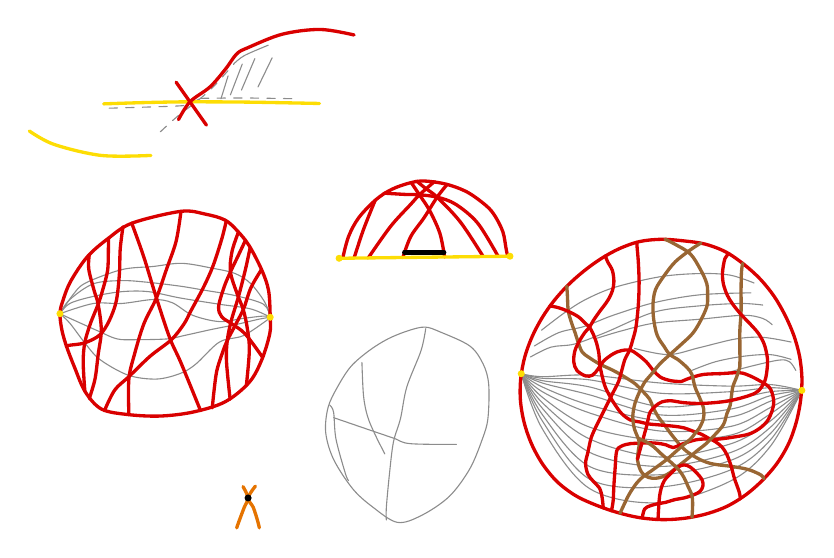
\begin{tikzpicture}[x=1mm,y=1mm,line cap=round,line join=round,font=\scriptsize]
\draw[pencil,dashed] plot[smooth, tension=0.3] coordinates {(11,-11.3) (16,-11.15) (20.6,-10.95) (22.6,-10.05)};
\draw[pencil,dashed] plot[smooth, tension=0.55] coordinates {(22.6,-10.05) (28,-10) (34.7,-10.1)};
\draw[pencil,dashed] plot[smooth, tension=0.55] coordinates {(17.5,-14.3) (19.6,-12.4) (22.6,-10.05) (24.5,-8.3) (26.9,-5.6)};
\draw[pencil] plot[smooth, tension=0.55] coordinates {(26.9,-5.6) (28.2,-4.6) (31.2,-3.3)};
\draw[pencil] (25.2,-10.1) -- (26.1,-7.2);
\draw[pencil] (26.4,-9.6) -- (27.9,-5.7);
\draw[pencil] (27.8,-9) -- (29.5,-5);
\draw[pencil] (29.9,-8.6) -- (31.7,-4.9);
\draw[Ye,very thick] plot[smooth, tension=0.55] coordinates {(10.3,-10.75) (15,-10.6) (20,-10.5) (25,-10.5) (30,-10.55) (37.7,-10.7)};
\draw[Rd,very thick] plot[smooth, tension=0.55] coordinates {(19.8,-12.75) (21.26,-10.49) (23.8,-8.6) (25.8,-6.3) (27.2,-4.4) (28.65,-3.6) (33,-1.9) (37.8,-1.3) (42.1,-2)};
\draw[Rd,very thick] (19.5,-8) -- (23.35,-13.45);
\draw[Ye,very thick] plot[smooth, tension=0.55] coordinates {(0.86,-14.2) (4,-15.9) (10,-17.3) (16.3,-17.3)};
\draw[pencil] plot[smooth, tension=0.55] coordinates {(4.75,-37.4) (6.4,-35) (8,-33.5) (12.6,-31.8) (16.6,-31.4) (20.2,-31) (24,-31.6) (27,-32.3) (29,-33.6) (30.8,-36) (31.45,-37.85)};
\draw[pencil] plot[smooth, tension=0.55] coordinates {(4.75,-37.4) (6,-35.6) (9,-33.6) (12.6,-33.2) (15.8,-33.4) (20,-33.9) (23,-34.4) (27,-35.1) (30.6,-36.2) (31.45,-37.85)};
\draw[pencil] plot[smooth, tension=0.55] coordinates {(4.75,-37.4) (6,-36.1) (9,-35.2) (12.6,-34.6) (16,-34.6) (20,-35.4) (25,-36.2) (29,-36.8) (31.45,-37.85)};
\draw[pencil] plot[smooth, tension=0.55] coordinates {(4.75,-37.4) (9,-36.1) (12.6,-36.1) (16.6,-35.6) (19,-36) (21.6,-37.6) (25,-38.4) (28,-38) (30.6,-37.7) (31.45,-37.85)};
\draw[pencil] plot[smooth, tension=0.55] coordinates {(4.75,-37.4) (5.6,-37.8) (9.6,-39.6) (12,-40.6) (14.4,-40.7) (18.4,-40.6) (20.4,-40.2) (24,-39.4) (27,-38.8) (30,-38.1) (31.45,-37.85)};
\draw[pencil] plot[smooth, tension=0.55] coordinates {(4.75,-37.4) (6,-38.6) (7.9,-41.1) (9.8,-43.2) (13.4,-45.2) (17,-45.7) (20,-45) (22,-43.8) (25,-41) (28,-40.2) (30.8,-38.4) (31.45,-37.85)};
\draw[Rd,very thick] plot[smooth cycle, tension=0.55] coordinates {(20.1,-24.4) (23.2,-24.75) (25.7,-25.5) (27.3,-26.9) (28.8,-28.8) (30.4,-31.9) (31.25,-34.5) (31.45,-37.85) (31.4,-39.9) (30.4,-43.2) (28.8,-46.1) (25.7,-48.6) (21.6,-49.9) (17.4,-50.4) (13.3,-50.2) (10,-49.5) (7.95,-47.3) (6.6,-44.2) (5.6,-41.6) (5,-39.5) (4.75,-37.4) (5.1,-35.8) (6.1,-33.3) (8.2,-30.2) (10.8,-27.9) (13.9,-25.9)};
\draw[Rd,very thick] plot[smooth, tension=0.55] coordinates {(8.48,-29.88) (8.4,-31.7) (9.1,-34.5) (9.6,-36.2) (10,-39.5) (9.6,-42.6) (9.2,-45.7) (8.47,-48.17)};
\draw[Rd,very thick] plot[smooth, tension=0.55] coordinates {(10.9,-27.82) (10.9,-29.2) (10.8,-31.9) (10.2,-34.3) (9.6,-36.2) (8.6,-38.7) (7.9,-41.1) (7.7,-43.6) (7.91,-47.24)};
\draw[Rd,very thick] plot[smooth, tension=0.55] coordinates {(12.75,-26.36) (12.4,-29.2) (12.3,-32.3) (11.9,-35.8) (11,-38.3) (9.8,-40.1) (7.9,-41.1) (6,-41.4) (5.56,-41.49)};
\draw[Rd,very thick] plot[smooth, tension=0.55] coordinates {(13.87,-25.91) (15.4,-30.2) (17,-35.4) (18.7,-40.5) (20.1,-43.6) (22.6,-49.7)};
\draw[Rd,very thick] plot[smooth, tension=0.55] coordinates {(20.12,-24.4) (19.5,-28.2) (18.3,-31.7) (17,-35.4) (15.4,-38.7) (14.2,-42.6) (13.5,-45.7) (13.5,-50.22)};
\draw[Rd,very thick] plot[smooth, tension=0.55] coordinates {(25.88,-25.59) (25.3,-27.9) (24.2,-31.3) (23,-34) (21.4,-37) (20.5,-38.7) (18.9,-40.7) (16.2,-42.8) (13.5,-45.4) (11.7,-47.1) (10.4,-49.71)};
\draw[Rd,very thick] plot[smooth, tension=0.55] coordinates {(27.42,-27.03) (26.6,-29.5) (26.4,-32.1) (27.3,-35) (28,-36.8) (28.5,-39) (28.8,-42) (28.42,-46.54)};
\draw[Rd,very thick] plot[smooth, tension=0.55] coordinates {(28.32,-28.05) (27.4,-30) (26.4,-32.1) (25.6,-34) (24.9,-36.5) (25.3,-37.8) (26.6,-38.7) (28.3,-40) (30.5,-42.96)};
\draw[Rd,very thick] plot[smooth, tension=0.55] coordinates {(28.91,-28.97) (28.3,-31.8) (27.4,-35.3) (26.5,-38.3) (26,-40.8) (25.9,-43.5) (26.36,-48.25)};
\draw[Rd,very thick] plot[smooth, tension=0.55] coordinates {(30.35,-31.78) (29,-34.1) (28.1,-36.7) (27.1,-38.7) (26,-40.8) (25.3,-42.6) (24.6,-45) (24.09,-49.36)};
\node[pt,Ye] at (4.75,-37.4) {};
\node[pt,Ye] at (31.45,-37.85) {};
\draw[Rd,very thick] plot[smooth, tension=0.55] coordinates {(42.1,-30.34) (43.3,-26.7) (44.78,-23)};
\draw[Rd,very thick] plot[smooth, tension=0.55] coordinates {(43.9,-30.32) (46.75,-26.3) (49.3,-23.5) (50.4,-22.3) (52.31,-20.62)};
\draw[Rd,very thick] plot[smooth, tension=0.55] coordinates {(48.3,-30.26) (49.3,-27.6) (51,-25.2) (52.65,-22.6) (53.92,-20.98)};
\draw[Rd,very thick] plot[smooth, tension=0.55] coordinates {(53.6,-30.2) (53,-27.2) (51.7,-24.3) (50.4,-22.3) (49.36,-20.74)};
\draw[Rd,very thick] plot[smooth, tension=0.55] coordinates {(58.5,-30.14) (55.6,-25.75) (52.65,-22.6) (51.2,-21.5) (50.04,-20.55)};
\draw[Rd,very thick] plot[smooth, tension=0.55] coordinates {(45.9,-22.09) (48.6,-22.25) (50.4,-22.3) (52.65,-22.6) (55,-23.5) (57.8,-25.9) (60.4,-30.12)};
\draw[Rd,very thick] plot[smooth, tension=0.55] coordinates {(40.66,-30.35) (41.4,-27.6) (42.7,-25.2) (44.9,-22.9) (46.9,-21.6) (49.15,-20.8) (51,-20.55) (53.8,-20.95) (56.5,-21.97) (58.9,-23.7) (60,-25) (61,-27) (61.4,-29.1) (61.6,-30.1)};
\draw[Ye,very thick] (40.2,-30.36) -- (61.9,-30.1);
\node[pt,Ye] at (40.2,-30.36) {};
\node[pt,Ye] at (61.9,-30.1) {};
\draw[black,line width=1.6pt] (48.48,-29.6) -- (53.54,-29.6);
\draw[pencil] plot[smooth cycle, tension=0.55] coordinates {(51.1,-39.1) (53,-39.7) (56.8,-41.5) (58.5,-43.8) (59.2,-46.4) (59.1,-50.7) (58.4,-53.3) (56.8,-57.1) (54.2,-60.6) (50.7,-63) (47.6,-63.9) (44.4,-61.9) (41.9,-59.6) (39.5,-55.9) (38.5,-52.5) (38.8,-49.3) (40,-46.7) (41.7,-44.1) (44,-42.1) (46.4,-40.6) (49,-39.55)};
\draw[pencil] plot[smooth, tension=0.55] coordinates {(51.2,-39.3) (50.6,-42.1) (48.8,-46.7) (48,-50.7) (47.1,-53.7) (46.6,-57.7) (46.2,-62) (46.2,-63.6)};
\draw[pencil] plot[smooth, tension=0.55] coordinates {(39.5,-50.6) (43,-51.8) (47.1,-53.2) (49.2,-53.9) (55.1,-54)};
\draw[pencil] plot[smooth, tension=0.55] coordinates {(43.1,-43.6) (43.3,-47.8) (43.8,-50.4) (44.7,-52.6) (46,-55.2)};
\draw[pencil] plot[smooth, tension=0.55] coordinates {(39,-49) (39.5,-49.9) (39.8,-53.3) (41,-57.7) (41.4,-58.6)};
\draw[pencil] plot[smooth, tension=0.55] coordinates {(65.9,-39.5) (68.8,-37.3) (71.5,-35.6) (75.2,-34.05) (81,-32.7) (86,-32.3) (89.85,-32.5) (92.9,-33.5)};
\draw[pencil] plot[smooth, tension=0.55] coordinates {(65,-41.5) (68.1,-39.8) (71.4,-39) (75,-37.6) (80.2,-36) (86,-35) (92.5,-34.75)};
\draw[pencil] plot[smooth, tension=0.55] coordinates {(64.5,-42.9) (67.1,-41.65) (70.1,-41.25) (74,-39.8) (80.2,-37.2) (86,-36.4) (91.2,-36.1) (94,-36.3)};
\draw[pencil] plot[smooth, tension=0.55] coordinates {(73,-40.5) (76,-39.6) (80.2,-38.6) (86,-38.1) (91.5,-37.6) (94,-38) (95.2,-38.8)};
\draw[pencil] plot[smooth, tension=0.55] coordinates {(77.7,-41.8) (82,-42.6) (86,-41.7) (90.6,-40.6) (94,-40.4) (97.6,-41)};
\draw[pencil] plot[smooth, tension=0.55] coordinates {(85,-44.6) (88,-43.5) (91.6,-42.8) (95,-42.6) (97.6,-43.2)};
\draw[pencil] plot[smooth, tension=0.55] coordinates {(88.5,-45.2) (92,-44.2) (96,-43.3) (97.4,-43.5) (98.2,-44.6)};
\draw[pencil] plot[smooth, tension=0.55] coordinates {(63.33,-45.02) (66,-45.4) (72,-45.2) (81,-46.2) (90,-46.6) (95,-46.4) (98.97,-47.14)};
\draw[pencil] plot[smooth, tension=0.55] coordinates {(63.33,-45.02) (66,-45.6) (72,-45.8) (81,-47.5) (90,-47.3) (95,-46.8) (98.97,-47.14)};
\draw[pencil] plot[smooth, tension=0.55] coordinates {(63.33,-45.02) (66,-45.9) (72,-46.7) (81,-49.2) (90,-48.3) (95,-47.3) (98.97,-47.14)};
\draw[pencil] plot[smooth, tension=0.55] coordinates {(63.33,-45.02) (66,-46.2) (72,-47.7) (81,-50.25) (90,-49.5) (95,-47.8) (98.97,-47.14)};
\draw[pencil] plot[smooth, tension=0.55] coordinates {(63.33,-45.02) (66,-46.7) (72,-49) (81,-51) (90,-50.5) (95,-48.5) (98.97,-47.14)};
\draw[pencil] plot[smooth, tension=0.55] coordinates {(63.33,-45.02) (66,-47.3) (72,-50) (81,-52.3) (90,-51.7) (95,-49.3) (98.97,-47.14)};
\draw[pencil] plot[smooth, tension=0.55] coordinates {(63.33,-45.02) (66,-48) (72,-51.8) (81,-53.5) (90,-52.8) (95,-50.1) (98.97,-47.14)};
\draw[pencil] plot[smooth, tension=0.55] coordinates {(63.33,-45.02) (66,-48.7) (72,-53.3) (81,-55.6) (90,-53.9) (95,-51) (98.97,-47.14)};
\draw[pencil] plot[smooth, tension=0.55] coordinates {(63.33,-45.02) (66,-49.4) (72,-55) (81,-56.8) (90,-55) (95,-51.8) (98.97,-47.14)};
\draw[pencil] plot[smooth, tension=0.55] coordinates {(63.33,-45.02) (66,-50.2) (72,-56.8) (81,-57.85) (90,-56) (95,-52.6) (98.97,-47.14)};
\draw[pencil] plot[smooth, tension=0.55] coordinates {(63.33,-45.02) (66,-51) (72,-58.4) (81,-59.4) (90,-57.2) (95,-53.4) (98.97,-47.14)};
\draw[pencil] plot[smooth, tension=0.55] coordinates {(63.33,-45.02) (66,-52) (72,-59.6) (81,-61.4) (90,-58.6) (95,-54.2) (98.97,-47.14)};
\draw[Rd,very thick] plot[smooth cycle, tension=0.55] coordinates {(63.27,-45.6) (63.79,-42.86) (64.73,-40.28) (65.99,-37.9) (67.51,-35.73) (69.27,-33.77) (71.24,-32.02) (73.39,-30.46) (75.76,-29.15) (78.35,-28.24) (81.1,-27.95) (83.87,-28.14) (86.64,-28.55) (89.28,-29.54) (91.61,-31.13) (93.69,-33.01) (95.44,-35.18) (96.83,-37.58) (97.94,-40.13) (98.68,-42.81) (98.98,-45.6) (98.81,-48.4) (98.26,-51.18) (97.31,-53.86) (95.87,-56.33) (94.01,-58.51) (91.85,-60.4) (89.4,-61.89) (86.71,-62.86) (83.92,-63.4) (81.1,-63.55) (78.3,-63.29) (75.56,-62.65) (72.88,-61.73) (70.26,-60.52) (67.93,-58.77) (66.06,-56.52) (64.66,-53.98) (63.71,-51.25) (63.23,-48.43)};
\draw[Br,very thick] plot[smooth, tension=0.55] coordinates {(69.12,-33.91) (69.2,-35.2) (69.3,-37) (69.7,-38.5) (70.2,-39.9) (70.6,-41.15) (71.1,-42.3) (72,-43) (73.3,-43.8) (75,-44.6) (76.25,-45.3) (77.8,-46.3) (78.75,-47.25) (79.6,-48.2) (80.15,-49.45) (80.8,-50.6) (81.5,-51.5) (82.3,-52.6) (83.1,-53.6) (83.6,-54.2) (84.3,-54.85) (85.1,-55.4) (86.2,-56) (87.3,-56.4) (88.4,-56.6) (90.1,-56.8) (92.2,-57.2) (93.8,-57.9) (94.15,-58.37)};
\draw[Rd,very thick] plot[smooth, tension=0.55] coordinates {(66.98,-36.4) (68.1,-36.65) (69.3,-37.1) (70.6,-37.8) (71.5,-38.65) (72,-39.1) (72.5,-40.05) (72.9,-41.15) (73.2,-42.5) (73.3,-43.8) (73.6,-45.3) (74,-46.7) (74.6,-47.9) (75.2,-48.9) (76.1,-50.1) (77.2,-50.9) (78.4,-51.15) (79.5,-51.4) (80.6,-51.5) (81.7,-51.6) (82.8,-51.7) (84,-51.9) (85.1,-52.3) (86.2,-52.7) (87.1,-53.2) (87.9,-53.6) (88.8,-54.3) (89.45,-55.3) (90,-56.8) (90.4,-58.3) (91,-60) (91.17,-60.9)};
\draw[Rd,very thick] plot[smooth, tension=0.55] coordinates {(74.01,-30.06) (74.3,-30.8) (74.9,-31.9) (75.1,-33.3) (74.9,-34.5) (74.3,-35.75) (73.3,-37.1) (72.5,-38.25) (72,-39.1) (71.4,-39.8) (70.7,-40.9) (70.15,-42.1) (70,-43.5) (70.4,-44.6) (71.5,-45.3) (72.4,-45.2) (73.1,-44.4) (73.8,-43.4) (75,-42.5) (76,-42.1) (77.1,-42) (78,-42.5) (79.2,-43.5) (80.1,-44.6) (81,-45.45) (82.3,-45.9) (83.7,-46) (84.4,-45.7) (85.3,-45.4) (86.6,-45.1) (88.8,-45) (91.1,-44.9) (92.4,-45.3) (93.75,-46) (94.8,-46.7) (95.2,-47.5) (95.4,-48.6) (95.2,-49.7) (94.6,-51) (93.55,-52) (92.2,-52.7) (90.1,-53.1) (88.1,-53.35) (86.8,-53.3) (85.6,-53.4) (84.5,-53.7) (83.4,-54.1) (82.6,-54.4) (81.7,-54.05) (80.6,-53.85) (79.5,-53.8) (78.4,-53.85) (77.2,-53.9) (76.1,-54.2) (75.45,-54.85) (75.25,-57.1) (75.1,-59.2) (75,-61.2) (74.79,-62.43)};
\draw[Rd,very thick] plot[smooth, tension=0.55] coordinates {(78.01,-28.32) (78.05,-29) (78.2,-30.8) (78.3,-33.5) (78.2,-36.3) (77.9,-39.1) (77.5,-40.7) (77.1,-42) (76.5,-43.2) (76.1,-44.6) (75.7,-46) (75,-47.4) (74.3,-48.8) (73.5,-50.4) (72.8,-51.8) (72.2,-53.2) (71.8,-55) (71.5,-56.4) (71.8,-57.8) (72.5,-58.7) (73.3,-59.6) (73.6,-60.7) (73.75,-62.08)};
\draw[Br,very thick] plot[smooth, tension=0.55] coordinates {(81.59,-27.94) (82.9,-28.6) (84.8,-29.8) (86.1,-31.8) (86.9,-33.6) (87,-35.2) (86.9,-36.5) (86.1,-38.3) (85.1,-39.9) (83.65,-41.3) (82.2,-42.6) (80.9,-43.8) (80.1,-44.8) (79,-46.1) (78.5,-47) (77.8,-48.7) (77.5,-50.4) (77.7,-52) (78.3,-53.6) (78.2,-54.8) (78.1,-56) (78.4,-57.1) (78.8,-57.75) (79.5,-58.2) (80.4,-58.3) (81.3,-58.1) (82.2,-57.6) (82.85,-57.1) (83.6,-56.5) (84.85,-55.5) (85.6,-54.85) (86.75,-53.95) (87.9,-52.8) (89,-51.5) (89.45,-50.1) (89.85,-49.1) (90,-48.1) (90.2,-46.7) (90.7,-45.4) (91.05,-44.3) (91.1,-43.8) (91.1,-41.6) (91.1,-39.4) (91.25,-37.2) (91.25,-34.3) (91.3,-32.1) (91.45,-31)};
\draw[Br,very thick] plot[smooth, tension=0.55] coordinates {(86.14,-28.43) (84.8,-29.3) (82.9,-30.8) (81.5,-32.55) (80.4,-34.3) (80.07,-36.1) (80.15,-38.1) (80.6,-40.15) (81.5,-41.6) (82.2,-42.6) (83.2,-43.2) (84.4,-44.25) (85,-45.1) (85.4,-46.7) (86,-48.1) (86.5,-49.5) (86.45,-50.8) (85.9,-52) (85.4,-52.6) (84.85,-53.3) (83.95,-54.05) (82.8,-55.05) (81.9,-55.85) (80.9,-56.6) (79.8,-57.4) (78.8,-58.1) (78,-58.9) (77,-60.4) (75.88,-62.74)};
\draw[Rd,very thick] plot[smooth, tension=0.55] coordinates {(89.7,-29.76) (89.2,-30.4) (88.9,-32.1) (89,-33.6) (89.5,-35.05) (90.2,-36.2) (91.25,-37.5) (92.4,-38.7) (93.45,-39.9) (94.2,-41.3) (94.6,-43.1) (94.55,-44.5) (94.25,-46) (93.45,-47.2) (92.4,-47.75) (90.5,-48.3) (88.8,-48.6) (86.2,-48.8) (84,-48.7) (82.3,-48.45) (81.2,-48.6) (80.4,-49.1) (79.7,-49.9) (79.45,-50.8) (79.25,-51.7) (79,-52.6) (78.75,-53.5) (78.09,-55.87)};
\draw[Rd,very thick] plot[smooth, tension=0.55] coordinates {(78.69,-63.35) (79,-62.2) (79.7,-61.8) (80.6,-61.55) (81.7,-61.35) (82.85,-61) (84,-60.8) (85.1,-60.45) (86,-60) (86.4,-59.3) (86.3,-58.5) (85.6,-57.6) (84.75,-56.85) (84,-56.6) (83.2,-56.9) (82.3,-57.7) (81.5,-58.6) (81.1,-59.6) (80.9,-60.6) (80.8,-61.8) (80.7,-63.54)};
\draw[Br,very thick] plot[smooth, tension=0.55] coordinates {(85.02,-63.26) (85.1,-61.55) (85,-60.45) (84.5,-59.3) (84,-58.2) (83.4,-57.3) (82.6,-56.5) (81.8,-55.8) (81,-55.1) (80.15,-54.3) (79.25,-53.7) (78.6,-53.4) (78.2,-53.22)};
\node[pt,Ye] at (63.33,-45.02) {};
\node[pt,Ye] at (98.97,-47.14) {};
\draw[Or,very thick] plot[smooth, tension=0.55] coordinates {(28,-59.36) (28.64,-60.8) (28.15,-62) (27.4,-64) (27.2,-64.6)};
\draw[Or,very thick] plot[smooth, tension=0.55] coordinates {(29.57,-59.3) (28.64,-60.8) (29.3,-62) (29.85,-63.7) (30.07,-64.6)};
\node[pt] at (28.64,-60.8) {};
\end{tikzpicture}
\end{document}
